\subsubsection{Uzunluk Teoremleri}
\begin{figure}[h!]
    \centering
    \begin{tikzpicture}
        \tkzDefPoint(0,0){A}
        \tkzDefPoint(2,2){C}
        \tkzDefPoint(3,0){B}
        
        \tkzDrawPolygon(A,B,C)
        \tkzDrawPoints(A,B,C)

        \tkzLabelPoints[below left](A)
        \tkzLabelPoints[above](C)
        \tkzLabelPoints[below right](B)

        \tkzLabelSegments[above right](B,C){$a$}
        \tkzLabelSegments[above left](A,C){$b$}
        \tkzLabelSegments[below](A,B){$c$}

        %---------------------------------------------------------------------------------
        
        \tkzDefPoint(6,0){D}
        \tkzDefPoint(8,2){E}
        \tkzDefPoint(9,0){F}
        
        \tkzDrawPolygon(D,F,E)
        \tkzDrawPoints(D,F,E)

        \tkzLabelPoints[below left](D)
        \tkzLabelPoints[above](E)
        \tkzLabelPoints[below right](F)

        \tkzLabelSegments[above right](F,E){$d$}
        \tkzLabelSegments[above left](D,E){$f$}
        \tkzLabelSegments[below](D,F){$e$}


    \end{tikzpicture}
    \caption{Benzer Üçgenler}
    \label{fig:simsegment}
\end{figure}

\ref{fig:simsegment} Benzer üçgenler figüründe de görülebileceği gibi $\widehat{ABC} \sim \widehat{DEF}$ geçerli ise, 
\begin{equation*}
    \begin{aligned}    
        \angle A = \angle D\text{, } \angle B = \angle E \text{, } \angle C = \angle F \\
        \frac{a}{d} = \frac{b}{e} = \frac{c}{f} = k \\
        \frac{n_a}{n_d} = \frac{n_b}{n_e} = \frac{n_c}{n_f} = k \\
        \frac{V_a}{V_d} = \frac{V_b}{V_e} = \frac{V_c}{V_f} = k \\
        \frac{h_a}{h_d} = \frac{h_b}{h_e} = \frac{h_c}{h_f} = k \\
        \text{Çevre}(ABC) = \text{Çevre}(DEF) = k \\
        \text{Alan}(ABC) = \text{Alan}(DEF) = k^2
    \end{aligned}
\end{equation*}
sağlanır.